%%%%%%%%%%%%%%%%%%%%%%%
%%  Capítulo 4: Estudio y diseño de la antena  %%
%%%%%%%%%%%%%%%%%%%%%%%

%%%%
\section{Parámetros de iluminación del reflector}
\label{sec_estudio_param}
%%%%

Para definir la antena que será utilizada como alimentador y sus respectivas dimensiones, es necesario en primer lugar conocer las dimensiones del reflector parabólico para poder determinar el diagrama de radiación del alimentador que se ajuste a lo pedido: EI = -11 dB, como se explicó en la sección \ref{subsec_principios_efi_glo_ilu}.

Las dimensiones del reflector parabólico son:
%%%%
\begin{align*}
D &= \text{1,8 m}\\
F &= \text{63,6 cm}\\
h_0 &= \text{31,8 cm}\\
r_0 &= \text{95,5 cm}\\
\theta_0 &= \text{71,5}^{\circ}\\
\dfrac{F}{D} &= \text{0,353}
\end{align*}
%%%%
A partir de la expresión \eqref{ec_principios:84}, la ganancia normalizada en dB en el ángulo $\theta_0$ queda expresada como:
%%%%
\begin{align}
{G_{fn}\left(\theta_0\right)}_{dB} = -11 \text{ dB} - P\!A
\label{ec_estudio:1}
\end{align}
%%%%
Considerando las dimensiones del reflector y empleando la ecuación \eqref{ec_principios:85}, la atenuación en el espacio libre producida por la diferencia de caminos $\Delta r$ resulta:
%%%%
\begin{align}
P\!A = 20\log\left(\dfrac{\text{63,6 cm}}{\text{95,5 cm}}\right)\Longrightarrow P\!A = -\text{3,5 dB}
\label{ec_estudio:2}
\end{align}
%%%%
y la expresión \eqref{ec_estudio:1} se reduce a:
%%%%
\begin{align}
{G_{fn}\left(\theta_0\right)}_{dB} = -\text{7,5 dB}
\label{ec_estudio:3}
\end{align}
%%%%
La antena que cumpla la función de alimentador debe generar una distribución espacial de campos tal que, para el ángulo $\theta_0$, la ganancia sea constante para todos los valores de $\upphi$ e igual a -7,5 dB, como puede observarse en el diagrama de radiación de la figura \ref{fig_estudio:1}.
%%%%
\begin{figure}[H]
\centering
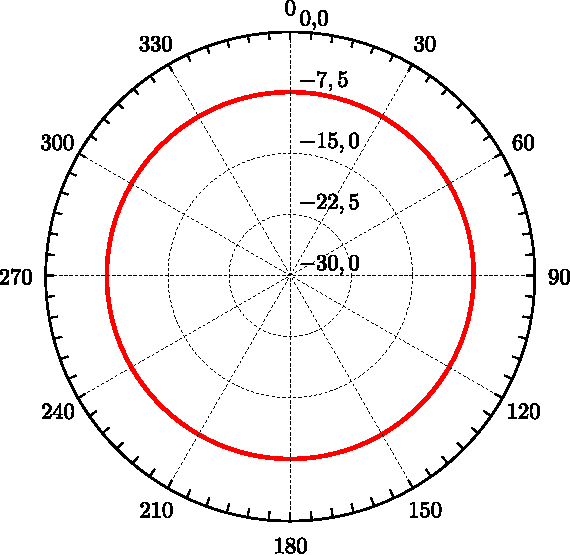
\includegraphics[scale = 1]{Figures/Estudio/estudio_1}
\caption{Diagrama de radiación del alimentador en el ángulo $\theta_0$.}
\label{fig_estudio:1}
\end{figure}
%%%%
A fin de determinar el alimentador requerido, se estudiaron las características de radiación de las siguientes antenas de abertura:
%%%%
\begin{itemize}
\item Abertura rectangular con plano conductor perfecto de extensión infinita y excitación con campo uniforme.
\item Abertura rectangular con plano conductor perfecto de extensión infinita y excitación con campo sinusoidal en modo dominante.
\item Abertura circular con plano conductor perfecto de extensión infinita y excitación con campo uniforme.
\item Abertura circular con plano conductor perfecto de extensión infinita y excitación con campo sinusoidal en modo dominante.
\item Guía de onda rectangular con extremo abierto.
\item Guía de onda cilíndrica con extremo abierto.
\item Bocina sectorial E.
\item Bocina sectorial H.
\item Bocina piramidal.
\item Bocina cónica.
\end{itemize}
%%%%
Para determinar las características de radiación de las antenas de abertura mencionadas anteriormente, se emplearon softwares de cálculo numérico (Matlab/Octave), a partir de las expresiones deducidas en los apéndices \ref{apendice_b} y \ref{apendice_c}. Para el caso de las antenas que sean excitadas con campo sinusoidal, se utilizan los modos dominantes, que corresponden al TE$_{10}$ para geometrías rectangulares y al TE$_{11}$ para geometrías circulares, cuyas expresiones han sido deducidas en el apéndice \ref{apendice_a}.

%%%%
\section{Aberturas con plano conductor perfecto de extensión infinita}
\label{sec_estudio_abert}
%%%%

Estas antenas son solamente modelos teóricos que se estudian con un fin didáctico previo al estudio de las antenas de abertura que son factibles de implementar en la práctica. La existencia de un plano conductor perfecto de extensión infinita concentra la radiación en valores de $\uptheta$ comprendidos entre 0$^{\circ}$ y 90$^{\circ}$.

%%%%
\subsection{Abertura rectangular con plano conductor perfecto de extensión infinita y excitación con campo uniforme}
\label{subsec_estudio_abert_rect_inf_uni}
%%%%

En la figura \ref{fig_estudio:2} se observa la geometría y las dimensiones de la abertura, y en las figuras \ref{fig_estudio:3} y \ref{grup_fig_estudio:1} se representan gráficamente los diagramas de radiación de la abertura con diferentes dimensiones, que se pueden observar en la tabla \ref{tabla_estudio:1}.
%%%%
\begin{figure}[H]
\centering
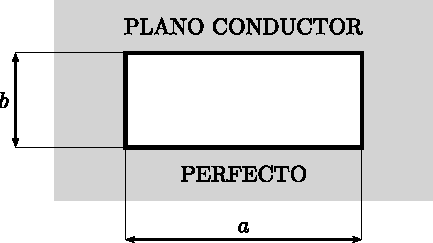
\includegraphics[scale = 1]{Figures/Estudio/estudio_2}
\caption{Dimensiones de la abertura rectangular con plano conductor perfecto de extensión infinita.}
\label{fig_estudio:2}
\end{figure}
%%%%
%%%%
\begin{figure}[H]
\centering
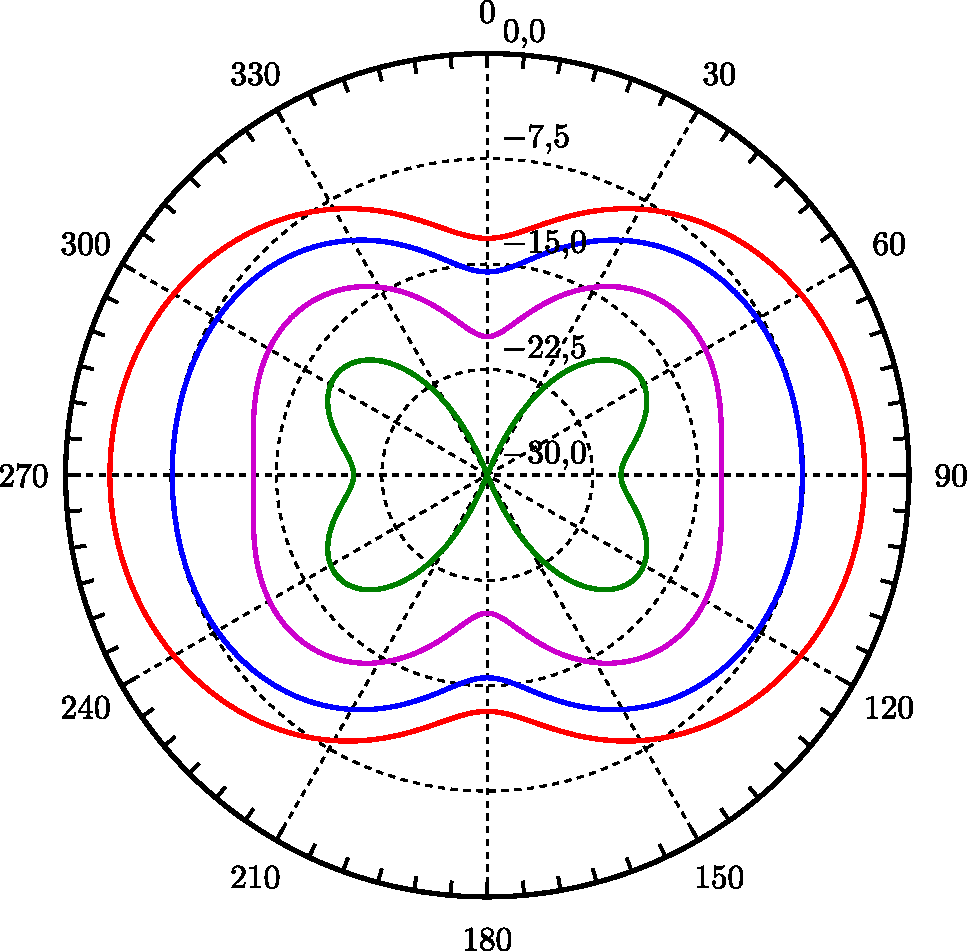
\includegraphics[scale = 0.5]{Figures/Estudio/estudio_3}
\caption{Diagramas de radiación en el ángulo $\theta_0$ de la abertura rectangular con plano conductor perfecto de extensión infinita y excitación con campo uniforme.}
\label{fig_estudio:3}
\end{figure}
%%%%
%%%%
\begin{figure} [H]
\centering 
\subfigure[Plano E.]{
\label{fig_estudio:4}
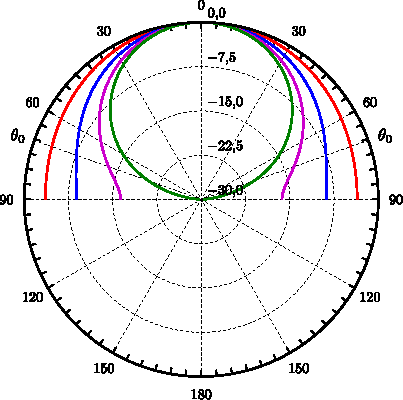
\includegraphics[scale = 1]{Figures/Estudio/estudio_4}}
\hspace{5mm}
\subfigure[Plano H.]{
\label{fig_estudio:5}
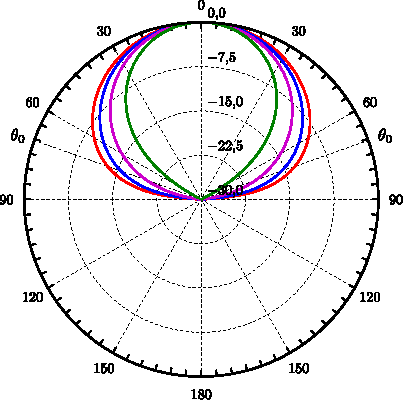
\includegraphics[scale = 1]{Figures/Estudio/estudio_5}}
\caption{Planos E y H de los diagramas de radiación de la abertura rectangular con plano conductor perfecto de extensión infinita y excitación con campo uniforme.}
\label{grup_fig_estudio:1}
\end{figure}
%%%%
\begin{table}[H]
\centering
\begin{tabular}{|c|c|c|c|c|c|}
\hline
\multirow{2}{*}{Trazo} & $a$ & $b$ & \multicolumn{2}{c|}{$G_{fn}\left(\theta_0\right)\,$(dB)} & $G_0$ \\
\cline{4-5}
& (mm) & (mm) & Plano E & Plano H & (dBi) \\
\hline

\includegraphics[scale = 1]{Figures/Estudio/linea_tabla_rojo} & 64,0 & 60,0 & -3,15 & -13,17 & 6,77 \\
\hline

\includegraphics[scale = 1]{Figures/Estudio/linea_tabla_azul} & 80,0 & 88,0 & -7,59 & -15,56 & 8,51 \\
\hline

\includegraphics[scale = 1]{Figures/Estudio/linea_tabla_violeta} & 100,0 & 108,0 & -13,35 & -20,16 & 10,16 \\
\hline

\includegraphics[scale = 1]{Figures/Estudio/linea_tabla_verde} & 132,0 & 121,0 & -20,49 & -56,65 & 11,80 \\
\hline
\end{tabular}
\caption{Ganancia normalizada en el ángulo $\theta_0$ y ganancia máxima de la abertura rectangular con plano conductor perfecto de extensión infinita y excitación con campo uniforme.}
\label{tabla_estudio:1}
\end{table}
%%%%

%%%%
\subsection{Abertura rectangular con plano conductor perfecto de extensión infinita y excitación con campo sinusoidal en modo dominante}
\label{subsec_estudio_abert_rect_inf_dom}
%%%%

En la figura \ref{fig_estudio:2} se observa la geometría y las dimensiones de la abertura, y en las figuras \ref{fig_estudio:6} y \ref{grup_fig_estudio:2} se representan gráficamente los diagramas de radiación de la abertura con diferentes dimensiones, que se pueden observar en la tabla \ref{tabla_estudio:2}.
%%%%
\begin{figure}[H]
\centering
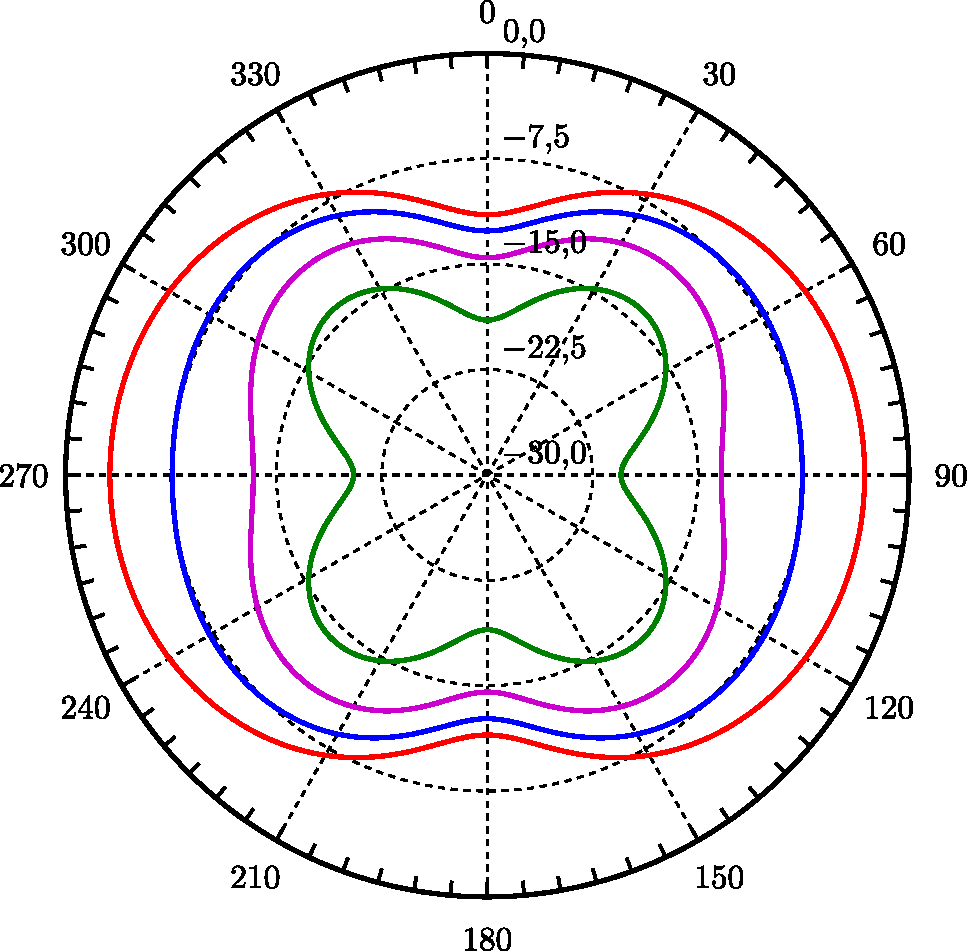
\includegraphics[scale = 0.5]{Figures/Estudio/estudio_6}
\caption{Diagramas de radiación en el ángulo $\theta_0$ de la abertura rectangular con plano conductor perfecto de extensión infinita y excitación con campo sinusoidal en modo dominante.}
\label{fig_estudio:6}
\end{figure}
%%%%
%%%%
\begin{figure} [H]
\centering 
\subfigure[Plano E.]{
\label{fig_estudio:7}
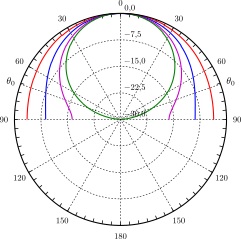
\includegraphics[scale = 1]{Figures/Estudio/estudio_7}}
\hspace{5mm}
\subfigure[Plano H.]{
\label{fig_estudio:8}
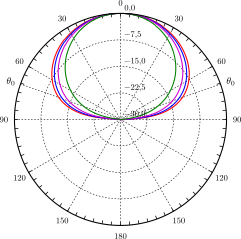
\includegraphics[scale = 1]{Figures/Estudio/estudio_8}}
\caption{Planos E y H de los diagramas de radiación de la abertura rectangular con plano conductor perfecto de extensión infinita y excitación con campo sinusoidal en modo dominante.}
\label{grup_fig_estudio:2}
\end{figure}
%%%%
\begin{table}[H]
\centering
\begin{tabular}{|c|c|c|c|c|c|}
\hline
\multirow{2}{*}{Trazo} & $a$ & $b$ & \multicolumn{2}{c|}{$G_{fn}\left(\theta_0\right)\,$(dB)} & $G_0$ \\
\cline{4-5}
& (mm) & (mm) & Plano E & Plano H & (dBi) \\
\hline

\includegraphics[scale = 1]{Figures/Estudio/linea_tabla_rojo} & 64,0 & 60,0 & -3,15 & -11,49 & 6,45 \\
\hline

\includegraphics[scale = 1]{Figures/Estudio/linea_tabla_azul} & 80,0 & 88,0 & -7,59 & -12,65 & 8,00 \\
\hline

\includegraphics[scale = 1]{Figures/Estudio/linea_tabla_violeta} & 100,0 & 108,0 & -13,35 & -14,55 & 9,40 \\
\hline

\includegraphics[scale = 1]{Figures/Estudio/linea_tabla_verde} & 132,0 & 121,0 & -20,49 & -18,98 & 10,73 \\
\hline
\end{tabular}
\caption{Ganancia normalizada en el ángulo $\theta_0$ y ganancia máxima de la abertura rectangular con plano conductor perfecto de extensión infinita y excitación con campo sinusoidal en modo dominante.}
\label{tabla_estudio:2}
\end{table}
%%%%

%%%%
\subsection{Abertura circular con plano conductor perfecto de extensión infinita y excitación con campo uniforme}
\label{subsec_estudio_abert_circ_inf_uni}
%%%%

En la figura \ref{fig_estudio:9} se observa la geometría y las dimensiones de la abertura, y en las figuras \ref{fig_estudio:10} y \ref{grup_fig_estudio:3} se representan gráficamente los diagramas de radiación de la abertura con diferentes dimensiones, que se pueden observar en la tabla \ref{tabla_estudio:3}.
%%%%
\begin{figure}[H]
\centering
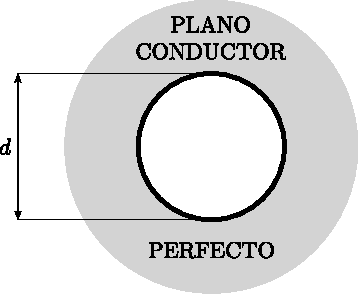
\includegraphics[scale = 1]{Figures/Estudio/estudio_9}
\caption{Dimensiones de la abertura circular con plano conductor perfecto de extensión infinita.}
\label{fig_estudio:9}
\end{figure}
%%%%
%%%%
\begin{figure}[H]
\centering
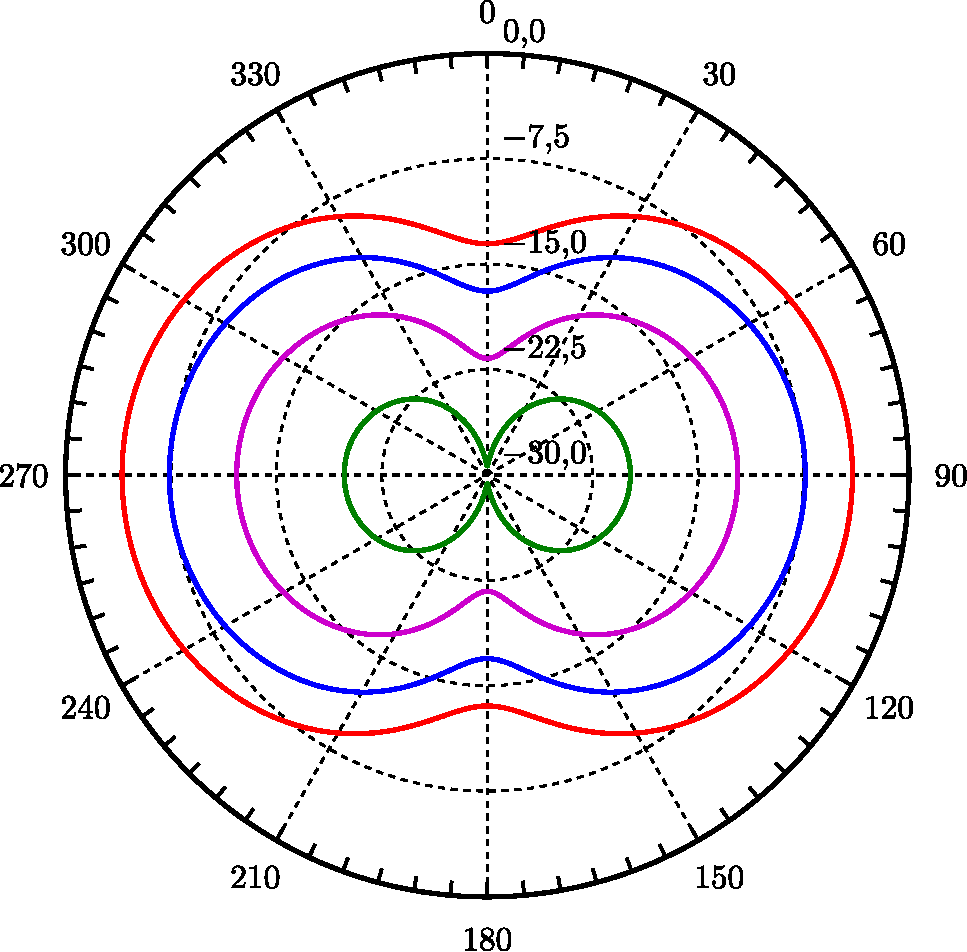
\includegraphics[scale = 0.5]{Figures/Estudio/estudio_10}
\caption{Diagramas de radiación en el ángulo $\theta_0$ de la abertura circular con plano conductor perfecto de extensión infinita y excitación con campo uniforme.}
\label{fig_estudio:10}
\end{figure}
%%%%
%%%%
\begin{figure} [H]
\centering 
\subfigure[Plano E.]{
\label{fig_estudio:11}
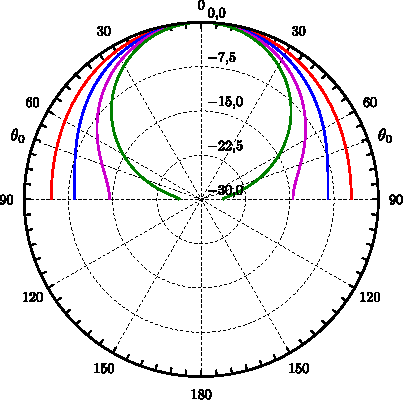
\includegraphics[scale = 1]{Figures/Estudio/estudio_11}}
\hspace{5mm}
\subfigure[Plano H.]{
\label{fig_estudio:12}
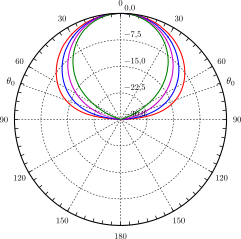
\includegraphics[scale = 1]{Figures/Estudio/estudio_12}}
\caption{Planos E y H de los diagramas de radiación de la abertura circular con plano conductor perfecto de extensión infinita y excitación con campo uniforme.}
\label{grup_fig_estudio:3}
\end{figure}
%%%%
\begin{table}[H]
\centering
\begin{tabular}{|c|c|c|c|c|}
\hline
\multirow{2}{*}{Trazo} & $d$ & \multicolumn{2}{c|}{$G_{fn}\left(\theta_0\right)\,$(dB)} & $G_0$ \\
\cline{3-4}
& (mm) & Plano E & Plano H & (dBi)\\
\hline

\includegraphics[scale = 1]{Figures/Estudio/linea_tabla_rojo} & 78,0 & -4,02 & -13,56 & 7,19 \\
\hline

\includegraphics[scale = 1]{Figures/Estudio/linea_tabla_azul} & 102,0 & -7,38 & -16,93 & 8,80 \\
\hline

\includegraphics[scale = 1]{Figures/Estudio/linea_tabla_violeta} & 124,0 & -12,17 & -21,72 & 10,43 \\
\hline

\includegraphics[scale = 1]{Figures/Estudio/linea_tabla_verde} & 144,0 & -19,82 & -29,36 & 11,84 \\
\hline
\end{tabular}
\caption{Ganancia normalizada en el ángulo $\theta_0$ y ganancia máxima de la abertura circular con plano conductor perfecto de extensión infinita y excitación con campo uniforme.}
\label{tabla_estudio:3}
\end{table}
%%%%

%%%%
\subsection{Abertura circular con plano conductor perfecto de extensión infinita y excitación con campo sinusoidal en modo dominante}
\label{subsec_estudio_abert_circ_inf_dom}
%%%%

En la figura \ref{fig_estudio:9} se observa la geometría y las dimensiones de la abertura, y en las figuras \ref{fig_estudio:13} y \ref{grup_fig_estudio:4} se representan gráficamente los diagramas de radiación de la abertura con diferentes dimensiones, que se pueden observar en la tabla \ref{tabla_estudio:4}.
%%%%
\begin{figure}[H]
\centering
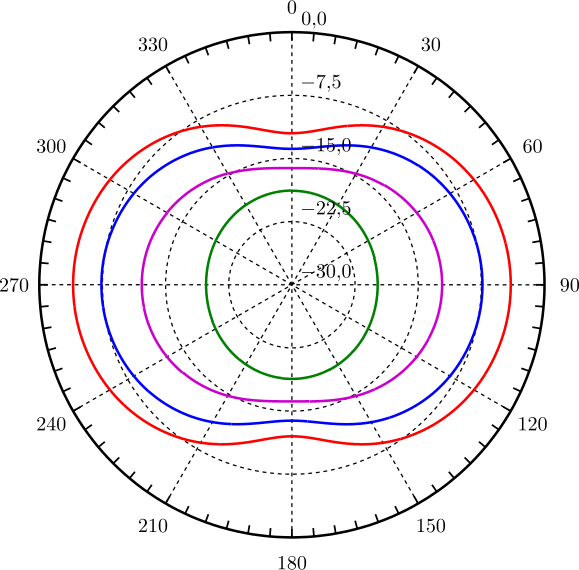
\includegraphics[scale = 0.5]{Figures/Estudio/estudio_13}
\caption{Diagramas de radiación en el ángulo $\theta_0$ de la abertura circular con plano conductor perfecto de extensión infinita y excitación con campo sinusoidal en modo dominante.}
\label{fig_estudio:13}
\end{figure}
%%%%
%%%%
\begin{figure} [H]
\centering 
\subfigure[Plano E.]{
\label{fig_estudio:14}
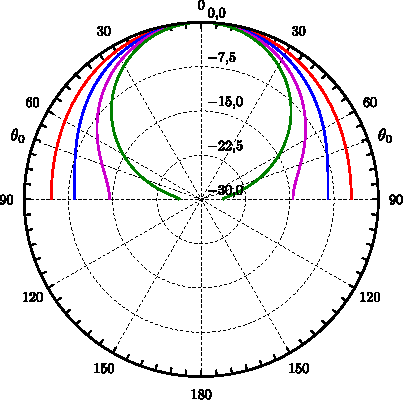
\includegraphics[scale = 1]{Figures/Estudio/estudio_14}}
\hspace{5mm}
\subfigure[Plano H.]{
\label{fig_estudio:15}
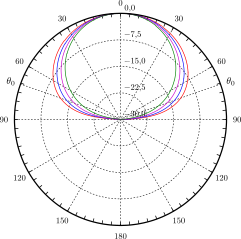
\includegraphics[scale = 1]{Figures/Estudio/estudio_15}}
\caption{Planos E y H de los diagramas de radiación de la abertura circular con plano conductor perfecto de extensión infinita y excitación con campo sinusoidal en modo dominante.}
\label{grup_fig_estudio:4}
\end{figure}
%%%%
\begin{table}[H]
\centering
\begin{tabular}{|c|c|c|c|c|}
\hline
\multirow{2}{*}{Trazo} & $d$ & \multicolumn{2}{c|}{$G_{fn}\left(\theta_0\right)\,$(dB)} & $G_0$ \\
\cline{3-4}
& (mm) & Plano E & Plano H & (dBi)\\
\hline

\includegraphics[scale = 1]{Figures/Estudio/linea_tabla_rojo} & 78,0 & -4,02 & -12,00 & 7,01 \\
\hline

\includegraphics[scale = 1]{Figures/Estudio/linea_tabla_azul} & 102,0 & -7,38 & -13,86 & 8,46 \\
\hline

\includegraphics[scale = 1]{Figures/Estudio/linea_tabla_violeta} & 124,0 & -12,17 & -16,15 & 9,89 \\
\hline

\includegraphics[scale = 1]{Figures/Estudio/linea_tabla_verde} & 144,0 & -19,82 & -18,84 & 11,12 \\
\hline
\end{tabular}
\caption{Ganancia normalizada en el ángulo $\theta_0$ y ganancia máxima de la abertura circular con plano conductor perfecto de extensión infinita y excitación con campo sinusoidal en modo dominante.}
\label{tabla_estudio:4}
\end{table}
%%%%

%%%%
\section{Guías de onda con extremo abierto}
\label{sec_estudio_guias}
%%%%

Estas antenas pueden dimensionarse para que se propague solamente el modo dominante y su centro de fase se ubica en el centro de la abertura, generando así, luego de la reflexión en la superficie metálica del paraboloide, una fase constante a través del plano de abertura. Las dimensiones de las guías de onda pueden incrementarse, en caso de ser necesario, siempre y cuando no se propaguen modos de orden superior que afecten el funcionamiento de la antena.

%%%%
\subsection{Guía de onda rectangular con extremo abierto}
\label{subsec_estudio_guia_rect}
%%%%

En la figura \ref{fig_estudio:16} se observa la geometría y las dimensiones de la guía de onda, y en las figuras \ref{fig_estudio:17} y \ref{grup_fig_estudio:5} se representan gráficamente los diagramas de radiación de la guía de onda con diferentes dimensiones, que se pueden observar en la tabla \ref{tabla_estudio:5}.
%%%%
\begin{figure}[H]
\centering
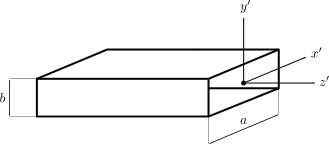
\includegraphics[scale = 1]{Figures/Estudio/estudio_16}
\caption{Dimensiones de la guía de onda rectangular con extremo abierto.}
\label{fig_estudio:16}
\end{figure}
%%%%
%%%%
\begin{figure}[H]
\centering
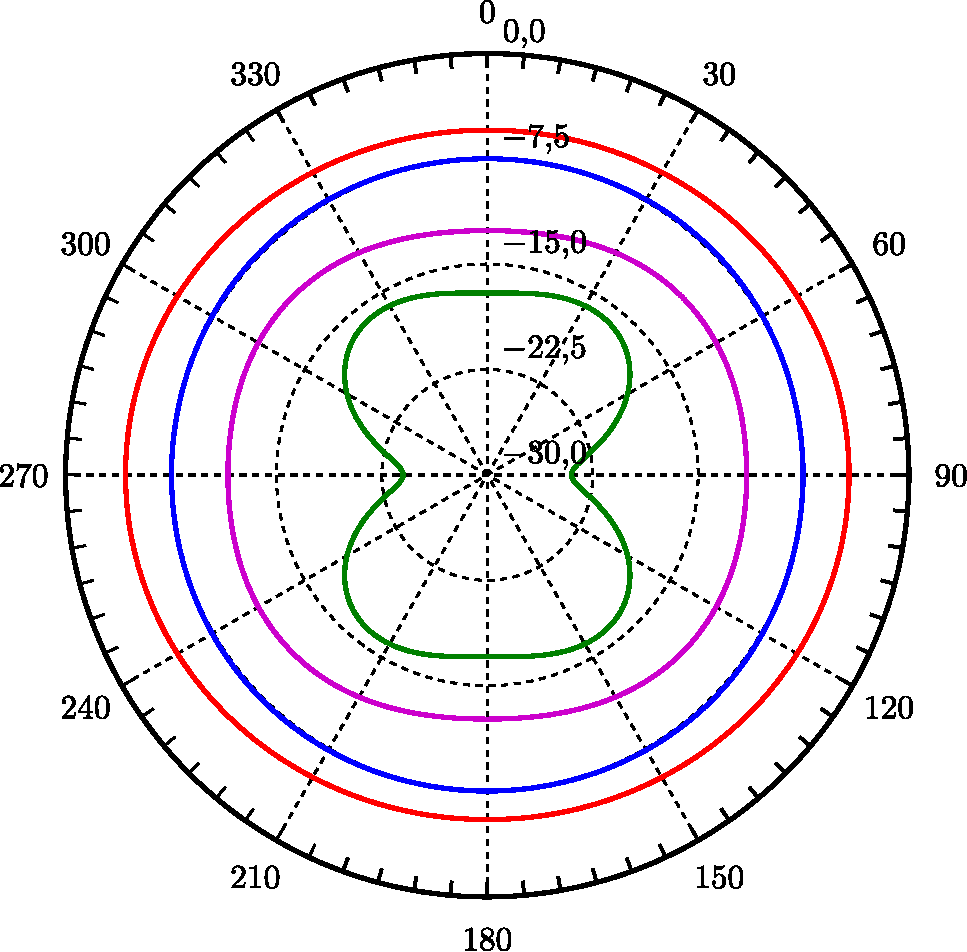
\includegraphics[scale = 0.5]{Figures/Estudio/estudio_17}
\caption{Diagramas de radiación en el ángulo $\theta_0$ de la guía de onda rectangular con extremo abierto.}
\label{fig_estudio:17}
\end{figure}
%%%%
%%%%
\begin{figure} [H]
\centering 
\subfigure[Plano E.]{
\label{fig_estudio:18}
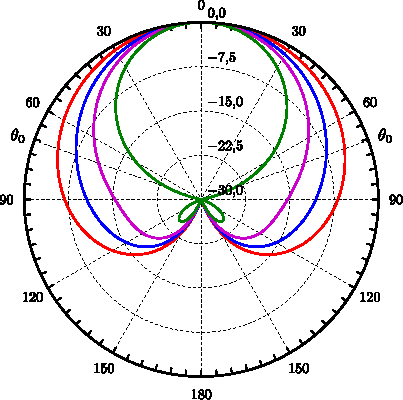
\includegraphics[scale = 1]{Figures/Estudio/estudio_18}}
\hspace{5mm}
\subfigure[Plano H.]{
\label{fig_estudio:19}
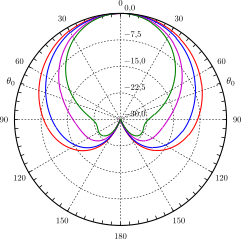
\includegraphics[scale = 1]{Figures/Estudio/estudio_19}}
\caption{Planos E y H de los diagramas de radiación de la guía de onda rectangular con extremo abierto.}
\label{grup_fig_estudio:5}
\end{figure}
%%%%
\begin{table}[H]
\centering
\begin{tabular}{|c|c|c|c|c|c|}
\hline
\multirow{2}{*}{Trazo} & $a$ & $b$ & \multicolumn{2}{c|}{$G_{fn}\left(\theta_0\right)\,$(dB)} & $G_0$ \\
\cline{4-5}
& (mm) & (mm) & Plano E & Plano H & (dBi)\\
\hline

\includegraphics[scale = 1]{Figures/Estudio/linea_tabla_rojo} & 64,0 & 30,0 & -4,27 & -5,47 & 5,64 \\
\hline

\includegraphics[scale = 1]{Figures/Estudio/linea_tabla_azul} & 90,0 & 67,0 & -7,54 & -7,51 & 7,17 \\
\hline

\includegraphics[scale = 1]{Figures/Estudio/linea_tabla_violeta} & 130,0 & 90,0 & -11,55 & -12,62 & 9,16 \\
\hline

\includegraphics[scale = 1]{Figures/Estudio/linea_tabla_verde} & 152,0 & 121,0 & -24,01 & -17,06 & 11,09 \\
\hline
\end{tabular}
\caption{Ganancia normalizada en el ángulo $\theta_0$ y ganancia máxima de la guía de onda rectangular con extremo abierto.}
\label{tabla_estudio:5}
\end{table}
%%%%

%%%%
\subsection{Guía de onda cilíndrica con extremo abierto}
\label{subsec_estudio_guia_cili}
%%%%

En la figura \ref{fig_estudio:20} se observa la geometría y las dimensiones de la guía de onda, y en las figuras \ref{fig_estudio:21} y \ref{grup_fig_estudio:6} se representan gráficamente los diagramas de radiación de la guía de onda con diferentes dimensiones, que se pueden observar en la tabla \ref{tabla_estudio:6}.
%%%%
\begin{figure}[H]
\centering
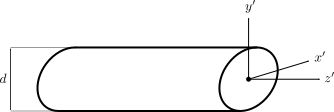
\includegraphics[scale = 1]{Figures/Estudio/estudio_20}
\caption{Dimensiones de la guía de onda cilíndrica con extremo abierto.}
\label{fig_estudio:20}
\end{figure}
%%%%
%%%%
\begin{figure}[H]
\centering
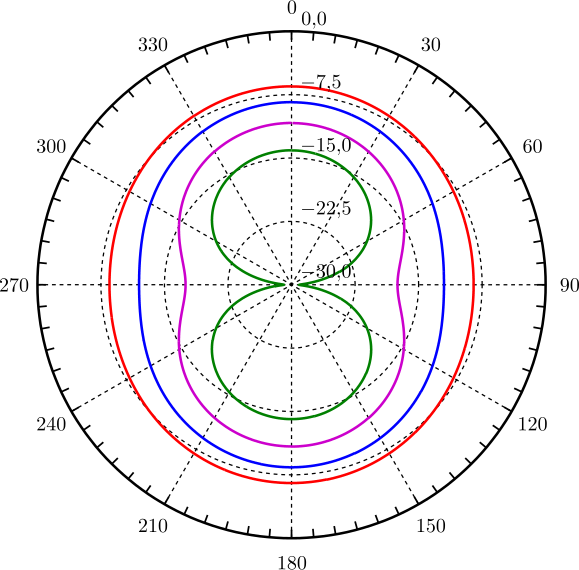
\includegraphics[scale = 0.5]{Figures/Estudio/estudio_21}
\caption{Diagramas de radiación en el ángulo $\theta_0$ de la guía de onda cilíndrica con extremo abierto.}
\label{fig_estudio:21}
\end{figure}
%%%%
%%%%
\begin{figure} [H]
\centering 
\subfigure[Plano E.]{
\label{fig_estudio:22}
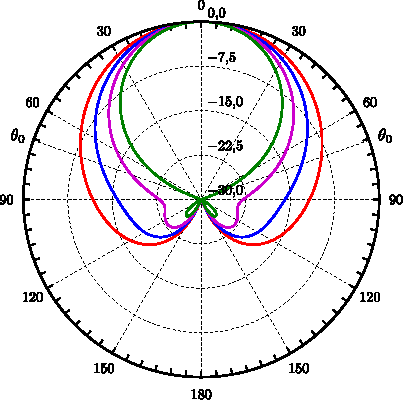
\includegraphics[scale = 1]{Figures/Estudio/estudio_22}}
\hspace{5mm}
\subfigure[Plano H.]{
\label{fig_estudio:23}
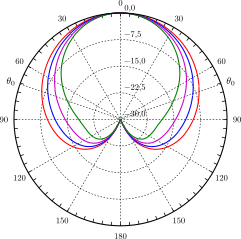
\includegraphics[scale = 1]{Figures/Estudio/estudio_23}}
\caption{Planos E y H de los diagramas de radiación de la guía de onda cilíndrica con extremo abierto.}
\label{grup_fig_estudio:6}
\end{figure}
%%%%
\begin{table}[H]
\centering
\begin{tabular}{|c|c|c|c|c|}
\hline
\multirow{2}{*}{Trazo} & $d$ & \multicolumn{2}{c|}{$G_{fn}\left(\theta_0\right)\,$(dB)} & $G_0$ \\
\cline{3-4}
& (mm) & Plano E & Plano H & (dBi)\\
\hline

\includegraphics[scale = 1]{Figures/Estudio/linea_tabla_rojo} & 86,0 & -8,51 & -6,53 & 7,15 \\
\hline

\includegraphics[scale = 1]{Figures/Estudio/linea_tabla_azul} & 108,0 & -12,00 & -8,40 & 8,39 \\
\hline

\includegraphics[scale = 1]{Figures/Estudio/linea_tabla_violeta} & 130,0 & -17,49 & -10,87 & 9,74 \\
\hline

\includegraphics[scale = 1]{Figures/Estudio/linea_tabla_verde} & 152,0 & -29,10 & -14,10 & 11,06 \\
\hline
\end{tabular}
\caption{Ganancia normalizada en el ángulo $\theta_0$ y ganancia máxima de la guía de onda cilíndrica con extremo abierto.}
\label{tabla_estudio:6}
\end{table}
%%%%

%%%%
\section{Bocinas}
\label{sec_estudio_bocinas}
%%%%

Las bocinas están compuestas básicamente por una guía de onda cuya sección se va incrementando paulatinamente hasta un extremo abierto, que se comporta como abertura. La guía de onda se dimensiona de forma tal que se propague solamente el modo dominante, y variando las dimensiones de la abertura es posible obtener la ganancia deseada sin que se propaguen otros modos, lo que constituye una clara ventaja respecto a las guías de onda con extremo abierto. No obstante, debido a que en la transición entre el extremo abierto de la guía de onda y la abertura se va incrementando la sección, el centro de fase no se ubicará en centro de la abertura, por lo que la fase a través del plano de abertura de las ondas radiadas, luego de reflejarse en el paraboloide, no será constante.

%%%%
\subsection{Bocina sectorial E}
\label{subsec_estudio_boci_sece}
%%%%

En las figuras \ref{fig_estudio:24} y \ref{fig_estudio:25} se observa la geometría y las dimensiones de la bocina, y en las figuras \ref{fig_estudio:26} y \ref{grup_fig_estudio:7} se representan gráficamente los diagramas de radiación de la bocina con diferentes dimensiones, que se pueden observar en la tabla \ref{tabla_estudio:7}.
%%%%
\begin{figure}[H]
\centering
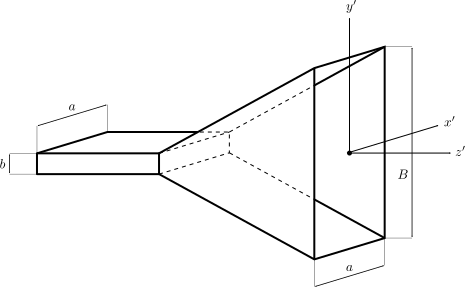
\includegraphics[scale = 1]{Figures/Estudio/estudio_24}
\caption{Dimensiones de la bocina sectorial E.}
\label{fig_estudio:24}
\end{figure}
%%%%
%%%%
\begin{figure}[H]
\centering
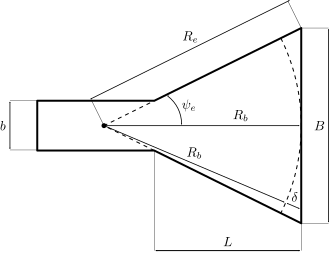
\includegraphics[scale = 1]{Figures/Estudio/estudio_25}
\caption{Corte en el plano E de la bocina sectorial E.}
\label{fig_estudio:25}
\end{figure}
%%%%
%%%%
\begin{figure}[H]
\centering
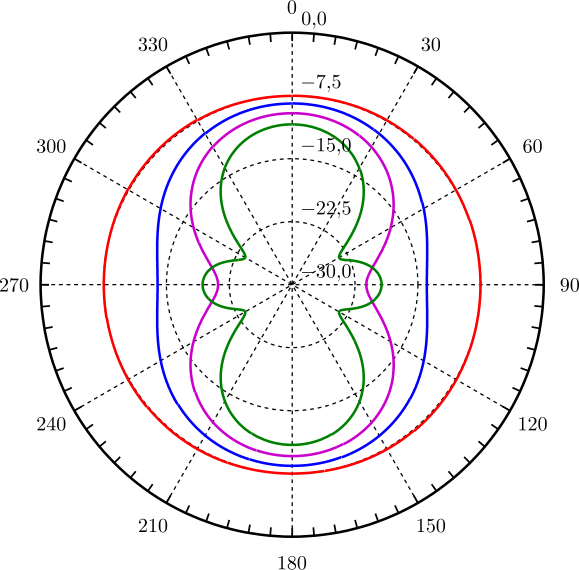
\includegraphics[scale = 0.5]{Figures/Estudio/estudio_26}
\caption{Diagramas de radiación en el ángulo $\theta_0$ de la bocina sectorial E.}
\label{fig_estudio:26}
\end{figure}
%%%%
%%%%
\begin{figure} [H]
\centering 
\subfigure[Plano E.]{
\label{fig_estudio:27}
\includegraphics[scale = 1]{Figures/Estudio/estudio_27}}
\hspace{5mm}
\subfigure[Plano H.]{
\label{fig_estudio:28}
\includegraphics[scale = 1]{Figures/Estudio/estudio_28}}
\caption{Planos E y H de los diagramas de radiación de la bocina sectorial E.}
\label{grup_fig_estudio:7}
\end{figure}
%%%%
\begin{table}[H]
\centering
\begin{tabular}{|c|c|c|c|c|c|c|c|}
\hline
\multirow{2}{*}{Trazo} & $a$ & $b$ & $B$ & $L$ & \multicolumn{2}{c|}{$G_{fn}\left(\theta_0\right)\,$(dB)} & $G_0$ \\
\cline{6-7}
& (mm) & (mm) & (mm) & (mm) & Plano E & Plano H & (dBi)\\
\hline
\includegraphics[scale = 1]{Figures/Estudio/linea_tabla_rojo} & 90,0 & 43,0 & 67,0 & 100,0 & -7,54 & -7,51 & 7,17 \\
\hline
\includegraphics[scale = 1]{Figures/Estudio/linea_tabla_azul} & 99,0 & 43,0 & 100,0 & 100,0 & -13,93 & -8,42 & 8,64 \\
\hline
\includegraphics[scale = 1]{Figures/Estudio/linea_tabla_violeta} & 109,0 & 55,0 & 120,0 & 120,0 & -21,17 & -9,58 & 9,69 \\
\hline
\includegraphics[scale = 1]{Figures/Estudio/linea_tabla_verde} & 119,0 & 55,0 & 150,0 & 150,0 & -19,32 & -10,92 & 10,91 \\
\hline
\end{tabular}
\caption{Ganancia normalizada en el ángulo $\theta_0$ y ganancia máxima de la bocina sectorial E.}
\label{tabla_estudio:7}
\end{table}
%%%%

%%%%
\subsection{Bocina sectorial H}
\label{subsec_estudio_boci_sech}
%%%%

En las figuras \ref{fig_estudio:29} y \ref{fig_estudio:30} se observa la geometría y las dimensiones de la bocina, y en las figuras \ref{fig_estudio:31} y \ref{grup_fig_estudio:8} se representan gráficamente los diagramas de radiación de la bocina con diferentes dimensiones, que se pueden observar en la tabla \ref{tabla_estudio:8}.
%%%%
\begin{figure}[H]
\centering
\includegraphics[scale = 1]{Figures/Estudio/estudio_29}
\caption{Dimensiones de la bocina sectorial H.}
\label{fig_estudio:29}
\end{figure}
%%%%
%%%%
\begin{figure}[H]
\centering
\includegraphics[scale = 1]{Figures/Estudio/estudio_30}
\caption{Corte en el plano H de la bocina sectorial H.}
\label{fig_estudio:30}
\end{figure}
%%%%
%%%%
\begin{figure}[H]
\centering
\includegraphics[scale = 0.5]{Figures/Estudio/estudio_31}
\caption{Diagramas de radiación en el ángulo $\theta_0$ de la bocina sectorial H.}
\label{fig_estudio:31}
\end{figure}
%%%%
%%%%
\begin{figure} [H]
\centering 
\subfigure[Plano E.]{
\label{fig_estudio:32}
\includegraphics[scale = 1]{Figures/Estudio/estudio_32}}
\hspace{5mm}
\subfigure[Plano H.]{
\label{fig_estudio:33}
\includegraphics[scale = 1]{Figures/Estudio/estudio_33}}
\caption{Planos E y H de los diagramas de radiación de la bocina sectorial H.}
\label{grup_fig_estudio:8}
\end{figure}
%%%%
\begin{table}[H]
\centering
\begin{tabular}{|c|c|c|c|c|c|c|c|}
\hline
\multirow{2}{*}{Trazo} & $a$ & $b$ & $A$ & $L$ & \multicolumn{2}{c|}{$G_{fn}\left(\theta_0\right)\,$(dB)} & $G_0$ \\
\cline{6-7}
& (mm) & (mm) & (mm) & (mm) & Plano E & Plano H & (dBi)\\
\hline
\includegraphics[scale = 1]{Figures/Estudio/linea_tabla_rojo} & 75,0 & 67,0 & 90,0 & 100,0 & -7,54 & -7,51 & 7,17 \\
\hline
\includegraphics[scale = 1]{Figures/Estudio/linea_tabla_azul} & 75,0 & 77,0 & 120,0 & 100,0 & -9,03 & -11,00 & 8,34 \\
\hline
\includegraphics[scale = 1]{Figures/Estudio/linea_tabla_violeta} & 109,0 & 87,0 & 150,0 & 120,0 & -10,90 & -16,38 & 9,61 \\
\hline
\includegraphics[scale = 1]{Figures/Estudio/linea_tabla_verde} & 109,0 & 97,0 & 200,0 & 150,0 & -13,29 & -24,46 & 11,23 \\
\hline
\end{tabular}
\caption{Ganancia normalizada en el ángulo $\theta_0$ y ganancia máxima de la bocina sectorial H.}
\label{tabla_estudio:8}
\end{table}
%%%%

%%%%
\subsection{Bocina piramidal}
\label{subsec_estudio_boci_pira}
%%%%

En las figuras \ref{fig_estudio:34}, \ref{fig_estudio:35} y \ref{fig_estudio:36} se observa la geometría y las dimensiones de la bocina, y en las figuras \ref{fig_estudio:37} y \ref{grup_fig_estudio:9} se representan gráficamente los diagramas de radiación de la bocina con diferentes dimensiones, que se pueden observar en la tabla \ref{tabla_estudio:9}.
%%%%
\begin{figure}[H]
\centering
\includegraphics[scale = 1]{Figures/Estudio/estudio_34}
\caption{Dimensiones de la bocina piramidal.}
\label{fig_estudio:34}
\end{figure}
%%%%
%%%%
\begin{figure}[H]
\centering
\includegraphics[scale = 1]{Figures/Estudio/estudio_35}
\caption{Corte en el plano E de la bocina piramidal.}
\label{fig_estudio:35}
\end{figure}
%%%%
%%%%
\begin{figure}[H]
\centering
\includegraphics[scale = 1]{Figures/Estudio/estudio_36}
\caption{Corte en el plano H de la bocina piramidal.}
\label{fig_estudio:36}
\end{figure}
%%%%
%%%%
\begin{figure}[H]
\centering
\includegraphics[scale = 0.5]{Figures/Estudio/estudio_37}
\caption{Diagramas de radiación en el ángulo $\theta_0$ de la bocina piramidal.}
\label{fig_estudio:37}
\end{figure}
%%%%
%%%%
\begin{figure} [H]
\centering 
\subfigure[Plano E.]{
\label{fig_estudio:38}
\includegraphics[scale = 1]{Figures/Estudio/estudio_38}}
\hspace{5mm}
\subfigure[Plano H.]{
\label{fig_estudio:39}
\includegraphics[scale = 1]{Figures/Estudio/estudio_39}}
\caption{Planos E y H de los diagramas de radiación de la bocina piramidal.}
\label{grup_fig_estudio:9}
\end{figure}
%%%%
%%%%
\begin{table}[H]
\centering
\begin{tabular}{|c|c|c|c|c|c|c|c|c|}
\hline
\multirow{2}{*}{Trazo} & $a$ & $b$ & $A$ & $B$ & $L$ & \multicolumn{2}{c|}{$G_{fn}\left(\theta_0\right)\,$(dB)} & $G_0$ \\
\cline{7-8}
& (mm) & (mm) & (mm) & (mm) & (mm) & Plano E & Plano H & (dBi)\\
\hline
\includegraphics[scale = 1]{Figures/Estudio/linea_tabla_rojo} & 75,0 & 43,0 & 90,0 & 67,0 & 100,0 & -7,54 & -7,51 & 7,17 \\
\hline
\includegraphics[scale = 1]{Figures/Estudio/linea_tabla_azul} & 86,0 & 43,0 & 120,0 & 90,0 & 100,0 & -11,49 & -11,02 & 8,86 \\
\hline
\includegraphics[scale = 1]{Figures/Estudio/linea_tabla_violeta} & 97,0 & 55,0 & 150,0 & 110,0 & 120,0 & -17,29 & -16,26 & 10,56 \\
\hline
\includegraphics[scale = 1]{Figures/Estudio/linea_tabla_verde} & 108,0 & 55,0 & 200,0 & 150,0 & 150,0 & -19,32 & -24,37 & 13,09 \\
\hline
\end{tabular}
\caption{Ganancia normalizada en el ángulo $\theta_0$ y ganancia máxima de la bocina piramidal.}
\label{tabla_estudio:9}
\end{table}
%%%%

%%%%
\subsection{Bocina cónica}
\label{subsec_estudio_boci_coni}
%%%%

En las figuras \ref{fig_estudio:40} y \ref{fig_estudio:41} se observa la geometría y las dimensiones de la bocina, y en las figuras \ref{fig_estudio:42} y \ref{grup_fig_estudio:10} se representan gráficamente los diagramas de radiación de la bocina con diferentes dimensiones, que se pueden observar en la tabla \ref{tabla_estudio:10}.
%%%%
\begin{figure}[H]
\centering
\includegraphics[scale = 1]{Figures/Estudio/estudio_40}
\caption{Dimensiones de la bocina cónica.}
\label{fig_estudio:40}
\end{figure}
%%%%
%%%%
\begin{figure}[H]
\centering
\includegraphics[scale = 1]{Figures/Estudio/estudio_41}
\caption{Corte longitudinal de la bocina cónica.}
\label{fig_estudio:41}
\end{figure}
%%%%
%%%%
\begin{figure}[H]
\centering
\includegraphics[scale = 0.5]{Figures/Estudio/estudio_42}
\caption{Diagramas de radiación en el ángulo $\theta_0$ de la bocina cónica.}
\label{fig_estudio:42}
\end{figure}
%%%%
%%%%
\begin{figure} [H]
\centering 
\subfigure[Plano E.]{
\label{fig_estudio:43}
\includegraphics[scale = 1]{Figures/Estudio/estudio_43}}
\hspace{5mm}
\subfigure[Plano H.]{
\label{fig_estudio:44}
\includegraphics[scale = 1]{Figures/Estudio/estudio_44}}
\caption{Planos E y H de los diagramas de radiación de la bocina cónica.}
\label{grup_fig_estudio:10}
\end{figure}
%%%%
%%%%
\begin{table}[H]
\centering
\begin{tabular}{|c|c|c|c|c|c|c|}
\hline
\multirow{2}{*}{Trazo} & $d$ & $D$ & $L$ & \multicolumn{2}{c|}{$G_{fn}\left(\theta_0\right)\,$(dB)} & $G_0$ \\
\cline{5-6}
& (mm) & (mm) & (mm) & Plano E & Plano H & (dBi)\\
\hline
\includegraphics[scale = 1]{Figures/Estudio/linea_tabla_rojo} & 80,0 & 86,0 & 100,0 & -8,51 & -6,53 & 7,15 \\
\hline
\includegraphics[scale = 1]{Figures/Estudio/linea_tabla_azul} & 84,0 & 136,0 & 100,0 & -18,97 & -11,63 & 10,08 \\
\hline
\includegraphics[scale = 1]{Figures/Estudio/linea_tabla_violeta} & 98,0 & 180,0 & 120,0 & -21,50 & -19,34 & 12,39 \\
\hline
\includegraphics[scale = 1]{Figures/Estudio/linea_tabla_verde} & 98,0 & 220,0 & 150,0 & -18,98 & -25,72 & 13,84 \\
\hline
\end{tabular}
\caption{Ganancia normalizada en el ángulo $\theta_0$ y ganancia máxima de la bocina cónica.}
\label{tabla_estudio:10}
\end{table}
%%%%

%%%%
\section{Selección del alimentador}
\label{sec_selec_alim}
%%%%

Para el reflector parabólico a utilizar, la relación $F/D$, como se vió en la sección \ref{sec_estudio_param}, es de 0,353. Descartadas las aberturas con plano conductor perfecto de extensión infinita por tratarse de modelos teóricos, la elección recae necesariamente en una guía de onda con extremo abierto o en una bocina. Como se ha visto en los diagramas de radiación en la sección \ref{sec_estudio_bocinas}, es posible dimensionar los distintos tipos de bocinas para obtener la iluminación deseada, según la expresión \eqref{ec_estudio:3}. Sin embargo, tal dimensionamiento implica que la abertura debe tener dimensiones similares a la guía de onda empleada en las bocinas.

Las guías de onda con extremo abierto también generan la iluminación deseada. Considerando las dimensiones de las guías de onda que cumplen con la condición de iluminación obtenidas de las tablas \ref{tabla_estudio:5} y \ref{tabla_estudio:6}, en la tabla \ref{tabla_estudio:11} se muestran las frecuencias de corte tanto para el modo dominante como para el siguiente modo de propagación.
%%%%
\begin{table}[H]
\centering
\begin{tabular}{|c|c|c|c|c|c|}
\hline
\multirow{2}{*}{Guía de} & \multirow{2}{*}{Dimensiones} & \multirow{2}{*}{Modo} & \multirow{2}{*}{1.$^{\text{er}}$ modo} & \multicolumn{1}{c|}{f$_\text{c}$ modo} & \multicolumn{1}{c|}{f$_\text{c}$ 1.$^{\text{er}}$ modo} \\
\multirow{2}{*}{onda} & \multirow{2}{*}{(mm)} & \multirow{2}{*}{dominante} & \multirow{2}{*}{superior} & dominante & superior \\
& & & & (GHz) & (GHz) \\
\hline
\multirow{2}{*}{Rectangular} & \multicolumn{1}{c|}{ancho = 90,0} & \multirow{2}{*}{TE$_{10}$} & \multirow{2}{*}{TE$_{01}$} & \multirow{2}{*}{1,67} & \multirow{2}{*}{2,24} \\
& alto = 67,0 & & & & \\
\hline
Cilíndrica & diámetro = 86,0 & TE$_{11}$ & TM$_{01}$ & 2,04 & 2,67 \\
\hline
\end{tabular}
\caption{Frecuencias de corte para el modo dominante y para el siguiente modo de propagación de las guías de onda con extremo abierto (ver apéndice \ref{apendice_a}  y \cite{Balaniselectro}).}
\label{tabla_estudio:11}
\end{table}
%%%%
Puede observarse que a la frecuencia de operación, la guía de onda rectangular propaga, además del modo dominante TE$_{10}$, el modo TE$_{01}$, mientras que la guía de onda cilíndrica propaga solamente el modo dominante TE$_{11}$.

Para determinar la distribuciones de campos generadas por los alimentadores estudiados, se ha empleado un método numérico basándose en la óptica geométrica: conociendo las densidades de corriente equivalentes sobre la abertura, se las integra para obtener los campos radiados. Un aspecto a considerar es que, al emplear este método para determinar los campos radiados, se asume que los campos eléctrico y mágnético sobre la abertura están relacionados como en una onda transverso-electromagnética ($\mathbf{TEM}$) \cite{Balanisantenas}:
%%%%
\begin{align}
\mathbf{H}_a \simeq \versor{n}\prodvec\dfrac{\mathbf{E}_a}{\eta}
\label{ec_estudio:4}
\end{align}
%%%%
Esta aproximación es válida en la medida que las dimensiones de la abertura sean lo suficientemente grandes como para considerar que los campos $\mathbf{E}_a$ y $\mathbf{H}_a$ constituyen una onda plana; en otras palabras, la aproximación es válida para aberturas con una ganancia moderada o alta. Claramente dicha aproximación pierde validez para las dimensiones de las guías de onda con extremo abierto necesarias para cumplir los parámetros de iluminación.

Un factor muy importante que la óptica geométrica no considera es la difracción producida en los bordes de los alimentadores; este fenómeno podrá alterar la distribución espacial de campos.

Para determinar la precisión con la que el modelo matemático predice la distribución de los campos radiados por ambas guías de onda, se realizaron simulaciones con el software FEKO para poder comparar los resultados obtenidos mediante la simulación con el método numérico basado en la óptica geométrica implementado con el software MATLAB/OCTAVE.

En las figuras \ref{fig_estudio:45} y \ref{grup_fig_estudio:12} se comparan los diagramas de radiación de la guía de onda rectangular con extremo abierto correspondientes al modelo teórico y a la simulación, y en la tabla \ref{tabla_estudio:12} se compara $G_{fn}\left(\theta_0\right)$ en los planos E y H y la ganancia máxima $G_0$.
%%%%
\begin{figure}[H]
\centering
\includegraphics[scale = 0.5]{Figures/Estudio/estudio_45}
\caption{Diagramas de radiación en el ángulo $\theta_0$ de la guía de onda rectangular con extremo abierto (modelo teórico y simulación).}
\label{fig_estudio:45}
\end{figure}
%%%%
%%%%
\begin{figure} [H]
\centering 
\subfigure[Plano E.]{
\label{fig_estudio:46}
\includegraphics[scale = 1]{Figures/Estudio/estudio_46}}
\hspace{5mm}
\subfigure[Plano H.]{
\label{fig_estudio:47}
\includegraphics[scale = 1]{Figures/Estudio/estudio_47}}
\caption{Planos E y H de los diagramas de radiación de la guía de onda rectangular con extremo abierto (modelo teórico y simulación).}
\label{grup_fig_estudio:12}
\end{figure}
%%%%
%%%%
\begin{table}[H]
\centering
\begin{tabular}{|c|c|c|c|c|c|c|}
\hline
\multirow{2}{*}{Método} & \multirow{2}{*}{Trazo} & $a$ & $b$ & \multicolumn{2}{c|}{$G_{fn}\left(\theta_0\right)\,$(dB)} & $G_0$ \\
\cline{5-6}
& & (mm) & (mm) & Plano E & Plano H & (dBi)\\
\hline
Modelo teórico & \includegraphics[scale = 1]{Figures/Estudio/linea_tabla_rojo} & 90,0 & 67,0 & -7,54 & -7,51 & 7,17 \\
\hline
Simulación & \includegraphics[scale = 1]{Figures/Estudio/linea_tabla_azul} & 90,0 & 67,0 & -6,66 & -12,46 & 7,72 \\
\hline
\end{tabular}
\caption{Ganancia normalizada en el ángulo $\theta_0$ y ganancia máxima de la guía de onda rectangular con extremo abierto (modelo teórico y simulación).}
\label{tabla_estudio:12}
\end{table}
%%%%
En las figuras \ref{fig_estudio:48} y \ref{grup_fig_estudio:13} se comparan los diagramas de radiación de la guía de onda cilíndrica con extremo abierto correspondientes al modelo teórico y a la simulación, y en la tabla \ref{tabla_estudio:13} se compara $G_{fn}\left(\theta_0\right)$ en los planos E y H y la ganancia máxima $G_0$.
%%%%
\begin{figure}[H]
\centering
\includegraphics[scale = 0.5]{Figures/Estudio/estudio_48}
\caption{Diagramas de radiación en el ángulo $\theta_0$ de la guía de onda cilíndrica con extremo abierto (modelo teórico y simulación).}
\label{fig_estudio:48}
\end{figure}
%%%%
%%%%
\begin{figure} [H]
\centering 
\subfigure[Plano E.]{
\label{fig_estudio:49}
\includegraphics[scale = 1]{Figures/Estudio/estudio_49}}
\hspace{5mm}
\subfigure[Plano H.]{
\label{fig_estudio:50}
\includegraphics[scale = 1]{Figures/Estudio/estudio_50}}
\caption{Planos E y H de los diagramas de radiación de la guía de onda cilíndrica con extremo abierto (modelo teórico y simulación).}
\label{grup_fig_estudio:13}
\end{figure}
%%%%
%%%%
\begin{table}[H]
\centering
\begin{tabular}{|c|c|c|c|c|c|}
\hline
\multirow{2}{*}{Método} & \multirow{2}{*}{Trazo} & $d$ & \multicolumn{2}{c|}{$G_{fn}\left(\theta_0\right)\,$(dB)} & $G_0$ \\
\cline{4-5}
& & (mm) & Plano E & Plano H & (dBi)\\
\hline
Modelo teórico & \includegraphics[scale = 1]{Figures/Estudio/linea_tabla_rojo} & 86,0 & -8,51 & -6,53 & 7,15 \\
\hline
Simulación & \includegraphics[scale = 1]{Figures/Estudio/linea_tabla_azul} & 86,0 & -8,36 & -9,43 & 7,59 \\
\hline
\end{tabular}
\caption{Ganancia normalizada en el ángulo $\theta_0$ y ganancia máxima de la guía de onda cilíndrica con extremo abierto (modelo teórico y simulación).}
\label{tabla_estudio:13}
\end{table}
%%%%
A partir de la comparaciones realizadas, puede observarse que mediante el modelo teórico puede obtenerse una buena aproximación de la ganancia máxima, pero debido a la difracción producida en los bordes de la abertura la distribución de campos no puede aproximarse con un error relativamente bajo; dicho efecto se evidencia fundamentalmente en el Plano H del diagrama de radiación y en la aparición de un lóbulo posterior.

En los diagramas de radiación de las figuras \ref{fig_estudio:45} - \ref{grup_fig_estudio:13} se evidencia que la guía de onda cilíndrica es menos afectada por la difracción que la guía de onda rectangular; en otras palabras, la distribución de campos generada por la guía de onda cilíndrica es la que más se acerca a los parámetros de iluminación deseados. Además, la guía de onda cilíndrica no permite la propagación de modos de orden superior a la frecuencia de operación. Por lo tanto, se concluye que la guía cilíndrica con extremo abierto es la estructura que mejor se ajusta a los parámetros de iluminación deseados.

Empleando el software de simulación, se redimensiona la guía de onda cilíndrica con extremo abierto para obtener la iluminación deseada. Para un diámetro de 83 mm, los diagramas de radiación obtenidos son los que se observan en las figuras \ref{fig_estudio:51} y \ref{grup_fig_estudio:14}.
%%%%
\begin{figure}[H]
\centering
\includegraphics[scale = 0.5]{Figures/Estudio/estudio_51}
\caption{Diagrama de radiación en el ángulo $\theta_0$ de la guía de onda cilíndrica con extremo abierto simulada, para un diámetro de 83 mm.}
\label{fig_estudio:51}
\end{figure}
%%%%
%%%%
\begin{figure} [H]
\centering 
\subfigure[Plano E.]{
\label{fig_estudio:52}
\includegraphics[scale = 1]{Figures/Estudio/estudio_52}}
\hspace{5mm}
\subfigure[Plano H.]{
\label{fig_estudio:53}
\includegraphics[scale = 1]{Figures/Estudio/estudio_53}}
\caption{Planos E y H del diagrama de radiación de la guía de onda cilíndrica con extremo abierto simulada, para un diámetro de 83 mm.}
\label{grup_fig_estudio:14}
\end{figure}
%%%%
Observando la figura \ref{fig_estudio:51}, puede decirse que una guía de onda cilíndrica con extremo abierto con un diámetro de 83 mm se ajusta satisfactoriamente a los parámetros de iluminación deseados. Sin embargo, debido a la difracción en el borde de la abertura se genera un lóbulo de radiación posterior, que se evidencia claramente en las figuras \ref{grup_fig_estudio:14}.

Con el fin de atenuar el lóbulo posterior, se estudia un alimentador que consiste en una guía de onda cilíndrica con extremo abierto y que posee una estructura anular cerca de la abertura, la cual se comporta como un choque. En la figura \ref{fig_estudio:54} puede observarse un gráfico de esta antena.
%%%%
\begin{figure}[H]
\centering
\includegraphics[scale = 1]{Figures/Estudio/estudio_54}
\caption{Guía de onda cilíndrica con choque anular.}
\label{fig_estudio:54}
\end{figure}
%%%%
Este tipo de antena puede tener no solamente un choque, sino dos, tres o más, y además, la longitud de los choques y la separación entre los mismos no debe ser necesariamente la misma \cite{James}. Debido a que una de las características deseadas del alimentador es que sus dimensiones sean lo más reducidas posibles para maximizar la eficiencia por bloqueo $\varepsilon_b$, se considera el estudio de la antena con un solo choque. En la figura \ref{fig_estudio:55} puede observarse un corte longitudinal de una guía de onda cilíndrica con sólo un choque.
%%%%
\begin{figure}[H]
\centering
\includegraphics[scale = 1]{Figures/Estudio/estudio_55}
\caption{Corte longitudinal de la guía de onda cilíndrica con un choque.}
\label{fig_estudio:55}
\end{figure}
%%%%
donde:
%%%%
\begin{align*}
d &= \text{Diámetro de la guía de onda cilíndrica.}\\
w &= \text{Ancho del choque.}\\
l &= \text{Longitud del choque.}\\
s &= \text{Separación entre el choque y la abertura de la antena.}
\end{align*}
%%%%
El choque presentará una reactancia a la onda de superficie que dependerá básicamente de su longitud. Asumiendo que el ancho del choque es mucho menor que la longitud de onda en el vacío (generalmente se considera $w < \lambda_0/10$), la reactancia del choque puede expresarse aproximadamente como \cite{Elliott}:
%%%%
\begin{align}
X = \eta_0\tan\left(kl\right)
\label{ec_estudio:5}
\end{align}
%%%%
Si se toma que la longitud del choque $l = \lambda_0/4$, la expresión \eqref{ec_estudio:5} se reduce a:
%%%%
\begin{align}
X = \eta_0\tan\left(\dfrac{2\pi}{ \lambda_0}\dfrac{\lambda_0}{4}\right) = \eta_0\tan\left(\dfrac{\pi}{2}\right)\longrightarrow\infty
\label{ec_estudio:6}
\end{align}
%%%%
Si la reactancia que presenta el choque a la onda de superficie es infinita, es de esperarse una disminución de la amplitud del lóbulo posterior, por lo tanto, se adopta $l$ = $\lambda_0/4$. La separación óptima entre el choque y la abertura de la antena es empírica, ya que no puede determinarse mediante un modelo matemático; lo mismo sucede con el ancho del choque.

Respecto al diámetro de la guía de onda cilíndrica, se adquirió un cilindro de latón de diámetro externo 82,6 mm y espesor 3 mm, el cual se ha torneado para obtener un diámetro interno mayor al original con el objetivo de alejar lo más posible la frecuencia de operación de la frecuencia de corte; el valor obtenido resultó $d$ = 79,2 mm.

Las dimensiones de $w$ y $s$ se han obtenido mediante simulación numérica.

Las dimensiones finales resultaron:
%%%%
\begin{align*}
d &= \text{79,2 mm}\\
w &= \text{11,0 mm}\\
l &= \text{31,2 mm}\\
s &= \text{31,2 mm}
\end{align*}    
%%%%
En las figuras \ref{fig_estudio:56} y \ref{grup_fig_estudio:15} se observan los diagramas de radiación obtenidos de la simulación de las guías de onda cilíndricas sola y con el agregado del choque para poder ver las mejoras.
%%%%
\begin{figure}[H]
\centering
\includegraphics[scale = 0.5]{Figures/Estudio/estudio_56}
\caption{Diagramas de radiación simulados en el ángulo $\theta_0$ de la guía de onda cilíndrica con y sin el choque.}
\label{fig_estudio:56}
\end{figure}
%%%%
%%%%
\begin{figure} [H]
\centering 
\subfigure[Plano E.]{
\label{fig_estudio:57}
\includegraphics[scale = 1]{Figures/Estudio/estudio_57}}
\hspace{5mm}
\subfigure[Plano H.]{
\label{fig_estudio:58}
\includegraphics[scale = 1]{Figures/Estudio/estudio_58}}
\put(-273,-45){\includegraphics[scale = 1]{Figures/Estudio/guia_con_sin_choque}}
\caption{Planos E y H de los diagramas de radiación simulados de la guía de onda cilíndrica con y sin el choque.}
\label{grup_fig_estudio:15}
\end{figure}
%%%%
En la tabla \ref{tabla_estudio:15} se muestra un cuadro comparativo con los parámetros de iluminación obtenidos por simulación para comparar el desempeño de la guía de onda cilíndrica cuando lleva el choque y cuando no lo lleva.
%%%%
\begin{table}[H]
\centering
\begin{tabular}{|c|c|c|c|c|}
\hline
Tipo de & \multicolumn{2}{c|}{$G_{fn}\left(\theta_0\right)\,$(dB)} & $G_0$ & Diferencia entre los lóbulos\\
\cline{2-3}
alimentador & Plano E & Plano H & (dBi) & principal y posterior (dB) \\
\hline
Guía de onda & \multirow{2}{*}{-7,64} & \multirow{2}{*}{-9,09} & \multirow{2}{*}{7,54} & \multirow{2}{*}{-10,91} \\
cilíndrica sin choque & & & & \\
\hline
Guía de onda & \multirow{2}{*}{-7,66} & \multirow{2}{*}{-9,02} & \multirow{2}{*}{7,57} & \multirow{2}{*}{-18,44} \\
cilíndrica con choque & & & & \\
\hline
\end{tabular}
\caption{Comparación de los parámetros principales entre la guía de onda cilíndrica con y sin el choque, obtenidos de la simulación.}
\label{tabla_estudio:15}
\end{table}
%%%%
Puede observarse en la tabla \ref{tabla_estudio:15} que la distribución de campos para ambos alimentadores es prácticamente la misma, con la excepción de la diferencia entre los lóbulos principal y posterior del diagrama de radiación. Al agregarse el choque, la amplitud del lóbulo posterior disminuye aproximadamente 7,5 dB, lo que constituye una clara mejora.

Con respecto a la eficiencia por bloqueo $\varepsilon_b$, se comparan las áreas proyetadas sobre el plano de abertura del reflector parabólico con la de ambos alimentadores para determinar la sombra que producen los alimentadores sobre el reflector.
%%%%
\begin{table}[H]
\centering
\begin{tabular}{|c|c|c|}
\hline
Tipo de & Área proyectada del & Área proyectada del\\
%\cline{2-3}
alimentador & alimentador (cm$^2$) & reflector sombreada (\%) \\
\hline
Guía de onda & \multirow{2}{*}{54,11} & \multirow{2}{*}{0,053} \\
cilíndrica sin choque & & \\
\hline
Guía de onda & \multirow{2}{*}{80,44} & \multirow{2}{*}{0,079} \\
cilíndrica con choque & & \\
\hline
\end{tabular}
\caption{Áreas proyectadas sobre el plano de abertura de la guía de onda cilíndrica con y sin el choque.}
\label{tabla_estudio:16}
\end{table}
%%%%
Puede verse en la tabla \ref{tabla_estudio:16} que la sombra que producen ambos alimentadores sobre el área proyectada del reflector en el plano de abertura es insignificante, lo que es de esperarse considerando que el diámetro del reflector es de 1,8 metros. Basándose en los resultados obtenidos, se concluye que la guía de onda cilíndrica con choque anular es la antena que mejor se adapta a los parámetros de iluminación deseados, por lo que es el alimentador que se escoge para su implementación.

%%%%
\section{Dimensionamiento del alimentador}
\label{sec_estudio_dimen}
%%%%

En la sección \ref{sec_selec_alim} se ha determinado que la guía de onda cilíndrica con choque anular es la antena que mejor se adapta a los pararámetros de iluminación deseados, y se dimensionó el diámetro de la guía de onda cilíndrica, el ancho y la longitud del choque y la separación entre el choque y la abertura de la antena; la dimensión que no se ha determinado es la longitud de la antena.

En las simulaciones del alimentador de la sección \ref{sec_selec_alim}, como la excitación de la antena se realizó asignando la distribución de campos en la guía de onda, que corresponde al modo de propagación dominante TE$_{11}$, la longitud del alimentador no influye en su desempeño. Al implementar el alimentador, hay que considerar dos aspectos: uno es que la atenuación que se produce en la guía de onda depende de la conductividad del material conductor con el que está construido el alimentador y de su longitud, y otro es que la excitación se realiza mediante una línea de transmisión coaxial a través de un conector N.

En la figura \ref{fig_estudio:59} puede verse un corte longitudinal del alimentador que es excitado mediante una línea de transmisión coaxial para la propagación del modo dominante con polarización vertical. En el interior de la guía de onda se encuentra un conductor de sección circular que funciona como excitador del alimentador.
%%%%
\begin{figure}[H]
\centering
\includegraphics[scale = 1]{Figures/Estudio/estudio_59}
\caption{Corte longitudinal del alimentador.}
\label{fig_estudio:59}
\end{figure}
%%%%
donde:
%%%%
\begin{align*}
L_e &= \text{Longitud del excitador.}\\
D_c &= \text{Distancia entre el excitador y el cortocircuito de la guía de onda.}\\
D_a &= \text{Distancia entre el excitador y la abertura de la guía de onda.}
\end{align*}
%%%%
Según la bibliografía consultada \cite{ARRL} \cite{Carr}, las dimensiones sugeridas de estos parámetros son:
%%%%
\begin{align*}
L_e &= \lambda_0/4\\
D_c &= \lambda_g/4\\
D_a &\geq \lambda_g/2
\end{align*}
%%%%
donde $\lambda_g$ es la longitud de onda en la guía de onda cilíndrica y cuya expresión, deducida en el apéndice \ref{apendice_a}, es:
%%%%
\begin{align}
&\lambda_g = \dfrac{\lambda_0}{\sqrt{1 - \left(\dfrac{f_c}{f}\right)^2}}
\label{ec_estudio:7}
\end{align}
%%%%
y $f_c$ es la frecuencia de corte, cuya expresión para una guía de onda cilíndrica y modo de propagación dominante, determinada en el apéndice \ref{apendice_a}, es:
%%%%
\begin{align}
&f_c = \frac{c}{\pi}\frac{\chi '_{11}}{d}
\label{ec_estudio:8}
\end{align}
%%%%
La distancia entre el excitador y la abertura $D_a$ se fija en $\lambda_g/2$ por una cuestión práctica: menor atenuación en la guía de onda y menos material a utilizarse. Con el fin de que los campos radiados en sentido al cortocircuito de la guía, luego de reflejarse en éste, generen una interferencia constructiva con los campos radiados en sentido a la abertura, se toma inicialmente que $D_c = \lambda_g/4$. Sin embargo, hay un aspecto que no se ha analizado hasta entonces: la impedancia que presenta el alimentador, que depende tanto de la longitud del excitador como de la distancia entre éste y el cortocircuito de la guía. Dado que una característica deseada de cualquier antena es que presente una ROE que sea lo más baja posible, para terminar de dimensionar el alimentador es necesario modificar tanto la longitud del excitador como la separación entre éste y el cortocircuito de la guía, para obetener una impedancia del alimentador que sea lo más cercana posible a 50 $\Omega$.

Empleando el software de simulación FEKO, se utilizó una herramienta llamada optimizador que dimensiona $L_e$ y $D_c$ en función de obtener la mínima ROE posible. Tomando que el diámetro del excitador es de 1 mm, se compara la ROE para los alimentadores simulados con dimensiones teóricas y optimizadas; se compara también la ganancia en la dirección principal de propagación $G_0$ para determinar si la variación de $D_c$ afecta la ganancia del alimentador.
%%%%
\begin{table}[H]
\centering
\begin{tabular}{|c|c|c|c|c|c|}
\hline
Dimensiones & $L_e$ (mm) & $D_c$ (mm) & $D_a$ (mm) & ROE & $G_0$ (dBi)\\
\hline
Teóricas & 31,2 & 81,8 & 163,7 & 1,32 & 7,41\\
\hline
Optimizadas & 29,2 & 42,3 & 163,7 & 1,05 & 7,41\\
\hline
\end{tabular}
\caption{ROE y $G_0$ obtenidas para el alimentador simulado con dimensiones teóricas y optimizadas.}
\label{tabla_estudio:17}
\end{table}
%%%%
En la tabla \ref{tabla_estudio:17} puede observarse que la ganancia del alimentador no se ve afectada al variar la posición del excitador respecto al cortocircuito de la guía de onda, pero la ROE se modifica logrando una adaptación muy cercana a la ideal; a la vez, la longitud del excitador varía muy poco respecto a la longitud teórica. A partir de estos resultados, se toman las dimensiones surgidas de la optimización como punto de partida en la implementación del alimentador; no obstante, tanto la longitud del excitador como la distancia entre éste y el cortocircuito de la guía de onda se ajustarán en la práctica en función de la medición de la ROE, lo que se verá detalladamente en la sección \ref{sec_resultados_med_imp_roe}.